\section{Einführung und Überblick}

\begin{definition}{Software Engineering}
\begin{itemize}
    \item \textbf{Disziplinen}: \\
    Anforderungen, Architektur, Implementierung, Test und Wartung
    \item \textbf{Ziel}: \\
    Strukturierte Prozesse für Qualität, Risiko- \& Fehlerminimierung
\end{itemize}
\end{definition}



\subsubsection{Softwareentwicklungsprozesse}

\begin{theorem}{Dimensionen Software-Entwicklungs-Probleme}
  \begin{itemize}
    \item Requirements (Bekannt - Unbekannt)
    \item Technology (Bekannt - Unbekannt)
    \item Skills/Experience (Vorhanden - Nicht vorhanden)
\end{itemize}
  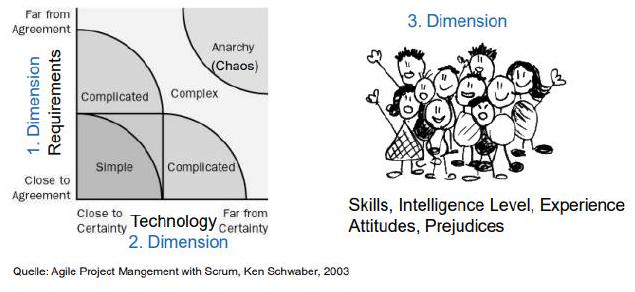
\includegraphics[width=\linewidth]{images/2024_12_29_0d1d7b5551ea1b4b41bdg-01}
\end{theorem}


\begin{corollary}{Kernprozesse}

\begin{minipage}[t]{0.6\textwidth}
\begin{itemize}
  \item Anforderungserhebung
  \item Systemdesign/technische Konzeption
  \item Implementierung
  \item Softwaretest
  \item Softwareeinführung
  \item Wartung/Pflege
\end{itemize}
\end{minipage}
\begin{minipage}[t]{0.38\textwidth}
\textbf{\textcolor{frog}{Unterstützungsprozesse}}
\begin{itemize}
  \item Projektmanagement
  \item Qualitätsmanagement
  \item Risikomanagement
\end{itemize}
\end{minipage}
\end{corollary}



\begin{concept}{Modelle in der Softwareentwicklung}
\begin{itemize}
  \item Software ist vielfach (immer?) selbst ein Modell
  \item Anforderungen sind Modelle der Problemstellung
  \item Architekturen und Entwürfe sind Modelle der Lösung
  \item Testfälle sind Modelle des korrekten Funktionierens des Codes usw.
\end{itemize}
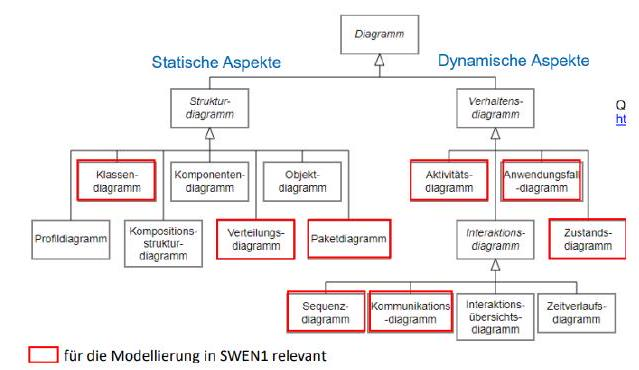
\includegraphics[width=\linewidth]{images/2024_12_29_0d1d7b5551ea1b4b41bdg-01(1)}
\end{concept}



\begin{formula}{Agile Softwareentwicklungsprozesse} Code and Fix\\
Vorgehen, bei dem Codierung oder Korrektur im Wechsel mit Ad-hoc-Tests die einzigen bewussten ausgeführten Tätigkeiten der Software-Entwicklung sind: Schnell, Agil, Einfach am Anfang, Schlecht Planbar, Schlecht Wartbar, Änderungen s. Aufwändig
\end{formula}

\begin{formula}{Wasserfallmodell}\\
Die Software-Entwicklung wird als Folge von Aktivitäten/Phasen betrachtet, die durch Teilergebnisse (Dokumente) gekoppelt sind. Die Reihenfolge der Ak-\\
tivitäten ist fest definiert. : gut planbar, klare Aufteilung in Phasen, Schlechtes Risikomanagment, nie alle Anforderungen zu Anfang bekannt
\end{formula}

\begin{formula}{Iterativ-inkrementelle Modelle}\\
Software wird in mehreren geplanten und kontrolliert durchgeführten Iterationen schrittweise (inkrementell) entwickelt: Flexibles Modell, Gutes Risikomanagement, Frühe Einsetzbarkeit, Planung upfront hat Grenzen, Kunde Involviert über ganze Entwicklung\\
Agile Softwareentwicklung Basiert auf interativ-inkrementellen Prozessmodell, Fokussiert auf gut dokumentierten und getesteten Code statt auf ausführlicher Dokumentation

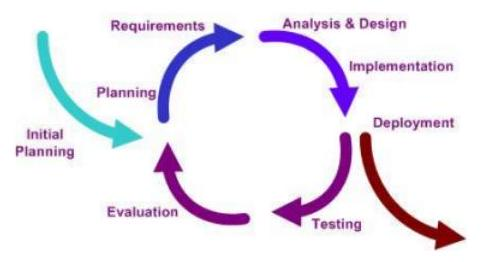
\includegraphics[width=0.8\linewidth]{images/2024_12_29_0d1d7b5551ea1b4b41bdg-02(1)}
\end{formula}


\begin{concept}{Charakteristiken iterativ-inkrementeller Prozesse}
\begin{itemize}
    \item Projekt-Abwicklung in Iterationen (Mini-Projekte)
    \item In jeder Iteration wird ein Stück der Software entwickelt (Inkrement)
    \item Ziele der Iterationen sind Risiko-getrieben
    \item Iterationen werden reviewed und die Learnings fliessen in die nächsten Iterationen ein
    \item Demming-Cycle: Plan, Do, Check, Act
\end{itemize}
\end{concept}

\begin{example2}{Typische Prüfungsaufgabe: Prozessmodelle vergleichen}\\
Vergleichen Sie das Wasserfallmodell mit einem iterativ-inkrementellen Ansatz anhand folgender Kriterien:
\begin{itemize}
    \item Umgang mit sich ändernden Anforderungen
    \item Risikomanagement
    \item Planbarkeit
    \item Kundeneinbindung
\end{itemize}

Musterlösung:
\begin{itemize}
    \item Wasserfall:
    \begin{itemize}
        \item Änderungen schwierig zu integrieren
        \item Risiken erst spät erkennbar
        \item Gut planbar durch feste Phasen
        \item Kunde hauptsächlich am Anfang und Ende involviert
    \end{itemize}
    \item Iterativ-inkrementell:
    \begin{itemize}
        \item Flexibel bei Änderungen
        \item Frühes Erkennen von Risiken
        \item Planung pro Iteration
        \item Kontinuierliches Kundenfeedback
    \end{itemize}
\end{itemize}
\end{example2}

\begin{concept}{Zweck und den Nutzen von Modellen in der Softwareentwicklung}\\
Modell von Requirements (close to/ far from Agreement) \& Technology (known / unknown)\\
Ein Modell ist ein konkretes oder gedankliches Abbild eines vorhanden Gebildes oder Vorbild für ein zu schaffendes Gebilde (hier Softwareprodukt).
\end{concept}

\begin{definition}{Begriffe}
  \begin{itemize}
    \item Warum wird modelliert: Um Analyse- und Designentwürfe zu diskutieren, abstimmen und zu dokumentieren bzw. zu kommunizieren.
    \item Modell: Ein Modell ist ein konkretes oder gedankliches Abbild eines vorhanden Gebildes oder Vorbild für ein zu schaffendes Gebilde (hier Softwareprodukt).
    \item Original: Das Original ist das abgebildete oder zu schaffende Gebilde.
    \item Modellierung: Modellierung gehört zum Fundament des Software Engineerings
  \end{itemize}
\end{definition}

\subsubsection{Modellierung}

\begin{definition}{Modellierung in der Softwareentwicklung}
\begin{itemize}
    \item Modelle als Abstraktionen: Anforderungen, Architekturen, Testfälle.
    \item Einsatz von UML: Skizzen, detaillierte Blueprints, vollständige Spezifikationen.
    \item Zweck:
    \begin{itemize}
        \item Verstehen eines Gebildes
        \item Kommunizieren über ein Gebilde
        \item Gedankliches Hilfsmittel zum Gestalten, Bewerten, Kritisieren
        \item Spezifikation von Anforderungen
        \item Durchführung von Experimenten
    \end{itemize}
\end{itemize}
\end{definition}

\begin{KR}{Modellierungsumfang bestimmen}
Folgende Fragen zur Bestimmung des notwendigen Modellierungsumfangs:
\begin{itemize}
    \item Wie komplex ist die Problemstellung?
    \item Wie viele Stakeholder sind involviert?
    \item Wie kritisch ist das System?
    \item Analogie: Planung einer Hundehütte vs. Haus vs. Wolkenkratzer
\end{itemize}
\end{KR}

\begin{example2}{Prüfungsfrage zur Modellierung}\\
Erklären Sie anhand eines selbst gewählten Beispiels, warum der Modellierungsaufwand je nach Projekt stark variieren kann. Nennen Sie mindestens drei Faktoren, die den Modellierungsumfang beeinflussen.
\vspace{3mm}\\
Mögliche Antwort:
\begin{itemize}
    \item Beispiel: Entwicklung einer Smartphone-App vs. Medizinisches Gerät
    \item Faktoren:
    \begin{itemize}
        \item Komplexität der Domäne
        \item Regulatorische Anforderungen
        \item Anzahl beteiligter Stakeholder
        \item Sicherheitsanforderungen
    \end{itemize}
\end{itemize}
\end{example2}

\begin{definition}{Unified Modelling Language (UML)}\\
UML ist die Standardsprache für die graphische Modellierung von Anforderungen, Analyse und Entwürfen im Software Engineering (objektorientierte Modellierung). (As a sketch, blueprint, programminglanguage)
\end{definition}

\begin{concept}{Basically}
\begin{itemize}
    \item Solide Analyse- und Entwurfskompetenzen sind essenziell.
    \item Iterativ-inkrementelle Modelle fördern agile Entwicklung.
\end{itemize}
\end{concept}

